\documentclass[article]{jss}
\usepackage{thumbpdf,listings} 
\graphicspath{{Figures/}}
\shortcites{sciencecloud,janus,dremel,nlme}

\DefineVerbatimEnvironment{example}{Verbatim}{}

\author{Dirk Eddelbuettel\\Debian Project \And 
        Murray Stokely\\Google, Inc \And
        Jeroen Ooms\\University of California,\\Los Angeles}
\Plainauthor{Dirk Eddelbuettel, Murray Stokely, Jeroen Ooms}

\title{\pkg{RProtoBuf}: Efficient Cross-Language Data Serialization in \proglang{R}}
\Plaintitle{RProtoBuf: Efficient Cross-Language Data Serialization in R}
\Shorttitle{\pkg{RProtoBuf}: Protocol Buffers in \proglang{R}}


\Abstract{
  Modern data collection and analysis pipelines often involve
  a sophisticated mix of applications written in general purpose and
  specialized programming languages.  Many formats commonly used to
  import and export data between different programs or systems, such
  as CSV or JSON, are verbose, inefficient, not
  type-safe, or tied to a specific programming language.  Protocol
  Buffers are a popular method of serializing structured data between
  applications -- while remaining independent of programming languages
  or operating systems.  They offer a unique combination of features,
  performance, and maturity that seems particularly well suited for
  data-driven applications and numerical computing.  The
  \pkg{RProtoBuf} package provides a complete interface to Protocol
  Buffers from the \proglang{R} environment for statistical computing.
  This paper outlines the general class of data serialization
  requirements for statistical computing, describes the implementation
  of the \pkg{RProtoBuf} package, and illustrates its use with example
  applications in large-scale data collection pipelines and web
  services.
}

\Keywords{\proglang{R}, \pkg{Rcpp}, Protocol Buffers, serialization, cross-platform}
\Plainkeywords{R, Rcpp, Protocol Buffers, serialization, cross-platform}

\Volume{71}
\Issue{2}
\Month{July}
\Year{2016}
\Submitdate{2014-02-05}
\Acceptdate{2015-04-13}
\DOI{10.18637/jss.v071.i02}

\Address{
  Dirk Eddelbuettel \\
  Debian Project \\
  River Forest, IL, United States of America\\
  E-mail: \email{edd@debian.org}\\
  URL: \url{http://dirk.eddelbuettel.com/}\\

  Murray Stokely\\
  Google, Inc.\\
  1600 Amphitheatre Parkway\\
  Mountain View, CA, United States of America\\
  E-mail: \email{murray@stokely.org}\\
  URL: \url{http://www.stokely.org/}\\

  Jeroen Ooms\\
  UCLA Department of Statistics\\
  University of California, Los Angeles\\
  Los Angeles, CA, United States of America\\
  E-mail: \email{jeroen.ooms@stat.ucla.edu}\\
  URL: \url{https://jeroenooms.github.io/}
}

\begin{document}

\vspace*{-0.3cm}

\section{Introduction} 

Modern data collection and analysis pipelines increasingly involve collections
of decoupled components in order to better manage software complexity 
through reusability, modularity, and fault isolation \citep{Wegiel:2010:CTT:1932682.1869479}.
These pipelines are frequently built using different programming 
languages for the different phases of data analysis -- collection,
cleaning, modeling, analysis, post-processing, and
presentation -- in order to take advantage of the unique combination of
performance, speed of development, and library support offered by
different environments and languages.  Each stage of such a data
analysis pipeline may produce intermediate results that need to be
stored in a file, or sent over the network for further processing. 

Given these requirements, how do we safely and efficiently share
intermediate results between different applications, possibly written
in different languages, and possibly running on different computer
systems?  In computer programming, \emph{serialization} is the process
of translating data structures, variables, and session states into a
format that can be stored or transmitted and then later reconstructed
in the original form \citep{clinec++}.  Programming languages such as
\proglang{R} \citep{r}, \proglang{Julia} \citep{julia},
\proglang{Java}, and \proglang{Python} \citep{python} include built-in
support for serialization, but the default formats are usually
language-specific and thereby lock the user into a single environment.

Data analysts and researchers often use character-separated text
formats such as CSV \citep{shafranovich2005common} to export
and import data. However, anyone who has ever used CSV files
will have noticed that this method has many limitations: It is
restricted to tabular data, lacks type-safety, and has limited
precision for numeric values.  Moreover, ambiguities in the format
itself frequently cause problems.  For example, conventions on which
characters are used as separator or decimal point vary by country.
\emph{Extensible markup language} (XML) is a well-established
and widely-supported format with the ability to define just about any
arbitrarily complex schema \citep{nolan2013xml}. However, it pays for
this complexity with comparatively large and verbose messages, and
added complexity at the parsing side (these problems are somewhat
mitigated by the availability of mature libraries and
parsers). Because XML is text-based and has no native notion of
numeric types or arrays, it is usually not a very practical format to
store numeric data sets as they appear in statistical applications.

A more modern format is \emph{\proglang{JavaScript} object notation}
(JSON), which is derived from the object literals of
\proglang{JavaScript}, and already widely-used on the world wide web.
Several \proglang{R} packages implement functions to parse and
generate JSON data from \proglang{R} objects
\citep{rjson,RJSONIO,jsonlite}.  JSON natively supports arrays
and four primitive types: numbers, strings, booleans, and
null. However, as it also is a text-based format, numbers are stored
in human-readable decimal notation which is inefficient and leads to
loss of type (double versus integer) and precision.  A number of
binary formats based on JSON have been proposed that reduce the
parsing cost and improve efficiency, but these formats are not widely
supported.  Furthermore, such formats lack a separate schema for the
serialized data and thus still duplicate field names with each message
sent over the network or stored in a file.

Once the data serialization needs of an application become complex
enough, developers typically benefit from the use of an
\emph{interface description language}, or \emph{IDL}.  IDLs like
Protocol Buffers \citep{protobuf}, Apache Thrift \citep{Apache:Thrift}, and Apache Avro \citep{Apache:Avro}
provide a compact well-documented schema for cross-language data
structures and efficient binary interchange formats.  Since the schema
is provided separately from the data, the data can be
efficiently encoded to minimize storage costs when
compared with simple ``schema-less'' binary interchange formats.
%Many sources compare data serialization formats
%and show Protocol Buffers perform favorably to the alternatives; see
%\citet{Sumaray:2012:CDS:2184751.2184810} for one such comparison.
Protocol Buffers perform well in the comparison of such formats by
\citet{Sumaray:2012:CDS:2184751.2184810}.

This paper describes an \proglang{R} interface to Protocol Buffers,
and is organized as follows. Section~\ref{sec:protobuf}
provides a general high-level overview of Protocol Buffers as well as a basic
motivation for their use.
Section~\ref{sec:rprotobuf-basic} describes the interactive \proglang{R} interface
provided by the \pkg{RProtoBuf} package, and introduces the two main abstractions:
\emph{Messages} and \emph{Descriptors}.  Section~\ref{sec:rprotobuf-classes}
details the implementation of the main \proglang{S}4 classes and methods.
Section~\ref{sec:types} describes the challenges of type coercion
between \proglang{R} and other languages.  Section~\ref{sec:evaluation} introduces a
general \proglang{R} language schema for serializing arbitrary \proglang{R} objects and compares it to
the serialization capabilities built directly into \proglang{R}.  Sections~\ref{sec:mapreduce}
and \ref{sec:opencpu} provide real-world use cases of \pkg{RProtoBuf}
in MapReduce and web service environments, respectively, before
Section~\ref{sec:summary} concludes.

\section{Protocol Buffers}
\label{sec:protobuf}

Protocol Buffers are a modern, language-neutral, platform-neutral,
extensible mechanism for sharing and storing structured data. Some of their
features, particularly in the context of data analysis, are:
%
\begin{itemize}
\item \emph{Portable}:  Enable users to send and receive data between
  applications as well as different computers or operating systems.
\item \emph{Efficient}:  Data is serialized into a compact binary
  representation for transmission or storage.
\item \emph{Extensible}:  New fields can be added to Protocol Buffer schemas
  in a forward-compatible way that does not break older applications.
\item \emph{Stable}:  Protocol Buffers have been in wide use for over a
  decade.
\end{itemize}
%
\begin{figure}[t!]
\centering
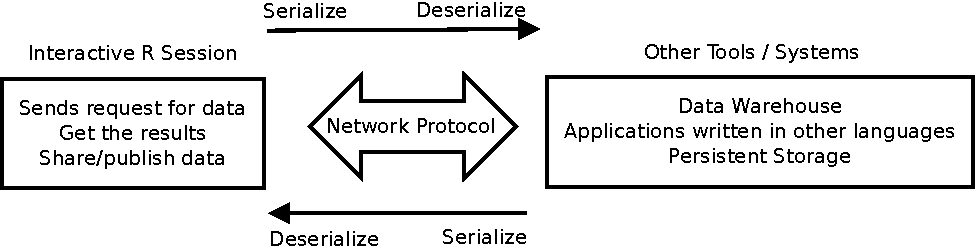
\includegraphics[width=0.9\textwidth]{protobuf-distributed-system-crop.pdf}
\caption{Example usage of Protocol Buffers.}
\label{fig:protobuf-distributed-usecase}
\end{figure}
%
Figure~\ref{fig:protobuf-distributed-usecase} illustrates an example
communication work flow with Protocol Buffers and an interactive \proglang{R} session.
Common use cases include populating a request remote-procedure call (RPC)
Protocol Buffer in \proglang{R} that is then serialized and sent over the network to a
remote server.  The server deserializes the message, acts on the
request, and responds with a new Protocol Buffer over the network.
The key difference to, say, a request to an \pkg{Rserve}
\citep{Urbanek:2003:Rserve,CRAN:Rserve} instance is that
the remote server may be implemented in any language.
%, with no dependence on \proglang{R}.

While traditional IDLs have at times been criticized for code bloat
and complexity, Protocol Buffers are based on a simple list and
records model that is flexible and easy to use.  The schema for
structured Protocol Buffer data is defined in \code{.proto} files,
which may contain one or more message types.  Each message type has
one or more fields.  A field is specified with a unique number (called
a \emph{tag number}), a name, a value type, and a field rule
specifying whether the field is optional, required, or repeated.  The
supported value types are numbers, enumerations, booleans, strings,
raw bytes, or other nested message types.  The \code{.proto} file
syntax for defining the structure of Protocol Buffer data is described
comprehensively on Google Code at
  \url{http://code.google.com/apis/protocolbuffers/docs/proto.html}.
Table~\ref{tab:proto} shows an example \code{.proto} file that defines
the \code{tutorial.Person} type\footnote{The compound name
  \code{tutorial.Person} in \proglang{R} is derived from the name of
  the message (\emph{Person}) and the name of the package defined at
  the top of the \code{.proto} file in which it is defined
  (\emph{tutorial}).}.  The \proglang{R} code in the right column
shows an example of creating a new message of this type and populating
its fields.

\begin{table}[t!]
\begin{tabular}{p{0.45\textwidth}p{0.5\textwidth}}
\hline
Schema : \code{addressbook.proto} & Example \proglang{R} session\\
\hline\\[-10pt]
\begin{minipage}{.40\textwidth}
\vspace{2mm}
\begin{example}
package tutorial;
message Person {
  required string name = 1;
  required int32 id = 2;
  optional string email = 3;
  enum PhoneType {
    MOBILE = 0; 
    HOME = 1;
    WORK = 2;
  }
  message PhoneNumber {
    required string number = 1;
    optional PhoneType type = 2;
  }
  repeated PhoneNumber phone = 4;
}
\end{example}
\vspace{2mm}
\end{minipage} & \begin{minipage}{.55\textwidth}
\begin{Schunk}
\begin{Sinput}
R> library("RProtoBuf")
R> p <- new(tutorial.Person, id = 1,
+    name = "Dirk")
R> p$name
\end{Sinput}
\begin{Soutput}
[1] "Dirk"
\end{Soutput}
\begin{Sinput}
R> p$name <- "Murray"
R> cat(as.character(p))
\end{Sinput}
\begin{Soutput}
name: "Murray"
id: 1
\end{Soutput}
\begin{Sinput}
R> serialize(p, NULL)
\end{Sinput}
\begin{Soutput}
 [1] 0a 06 4d 75 72 72 61 79 10 01
\end{Soutput}
\begin{Sinput}
R> class(p)
\end{Sinput}
\begin{Soutput}
[1] "Message"
attr(,"package")
[1] "RProtoBuf"
\end{Soutput}
\end{Schunk}
\vspace{0.5mm}
\end{minipage} \\
\hline
\end{tabular}
\caption{The schema representation from a \code{.proto} file for the
  \code{tutorial.Person} type (left) and simple \proglang{R} code for creating
  an object of this class and accessing its fields (right).}
\label{tab:proto}
\end{table}

For added speed and efficiency, the \proglang{C++}, \proglang{Java},
and \proglang{Python} bindings to
Protocol Buffers are used with a compiler that translates a Protocol
Buffer schema description file (ending in \code{.proto}) into
language-specific classes that can be used to create, read, write, and
manipulate Protocol Buffer messages.  The \proglang{R} interface, in contrast,
uses a reflection-based API that makes some operations slightly
slower but which is much more convenient for interactive data analysis.
All messages in \proglang{R} have a single class
structure, but different accessor methods are created at runtime based
on the named fields of the specified message type, as described in the
next section.

\section{Basic usage: Messages and descriptors}
\label{sec:rprotobuf-basic}

This section describes how to use the \proglang{R} API to create and manipulate
Protocol Buffer messages in \proglang{R}, and how to read and write the
binary representation of the message (often called the \emph{payload}) to files and arbitrary binary
\proglang{R} connections.
The two fundamental building blocks of Protocol Buffers are \emph{Messages}
and \emph{Descriptors}.  Messages provide a common abstract encapsulation of
structured data fields of the type specified in a Message Descriptor.
Message Descriptors are defined in \code{.proto} files and define a
schema for a particular named class of messages.

\subsection[Importing Message Descriptors from .proto files]{Importing
  Message Descriptors from \code{.proto} files}

To create or parse a Protocol Buffer message, one must first read in
the Message Descriptor (\emph{message type}) from a \code{.proto} file.
A small number of message types are imported when the package is first
loaded, including the \code{tutorial.Person} type we saw in the last
section.
All other types must be imported from
\code{.proto} files using the \code{readProtoFiles}
function, which can either import a single file, all files in a directory,
or every \code{.proto} file provided by a particular \proglang{R} package.

After importing proto files, the corresponding Message Descriptors are
available by name from the \code{RProtoBuf:DescriptorPool} environment
in the \proglang{R} search path.  This environment is implemented with
the user-defined tables framework from the \pkg{RObjectTables} package
available from the OmegaHat project \citep{RObjectTables}.  Instead of
being associated with a static hash table, this environment
dynamically queries the in-memory database of loaded descriptors
during normal variable lookup.  This allows new descriptors to be
parsed from \code{.proto} files and added to the global
namespace.\footnote{Note that there is a significant performance
  overhead with this \pkg{RObjectTables} implementation.  Because the
  table is on the search path and is not cacheable, lookups of symbols
  that are behind it in the search path cannot be added to the global
  object cache, and \proglang{R} must perform an expensive lookup
  through all of the attached environments and the Protocol Buffer
  definitions to find common symbols (most notably those in base) from
  the global environment.  Fortunately, proper use of namespaces and
  package imports reduces the impact of this for code in packages.}

\subsection{Creating, accessing, and modifying messages}

New messages are created with the \code{new} function which accepts
a Message Descriptor and optionally a list of ``name = value'' pairs
to set in the message.
%The objects contained in the special environment are
%descriptors for their associated message types. Descriptors will be
%discussed in detail in another part of this document, but for the
%purpose of this section, descriptors are just used with the \code{new}
%function to create messages.
%
\begin{Schunk}
\begin{Sinput}
R> p <- new(tutorial.Person, name = "Murray", id = 1)
\end{Sinput}
\end{Schunk}
%
Once the message is created, its fields can be queried
and modified using the dollar operator of \proglang{R}, making Protocol
Buffer messages seem like lists.
%
\begin{Schunk}
\begin{Sinput}
R> p$name
\end{Sinput}
\begin{Soutput}
[1] "Murray"
\end{Soutput}
\begin{Sinput}
R> p$id
\end{Sinput}
\begin{Soutput}
[1] 1
\end{Soutput}
\begin{Sinput}
R> p$email <- "murray@stokely.org"
\end{Sinput}
\end{Schunk}
%
As opposed to \proglang{R} lists, no partial matching is performed
and the name must be given entirely.
The \verb|[[| operator can also be used to query and set fields
of a message, supplying either their name or their tag number:
%
\begin{Schunk}
\begin{Sinput}
R> p[["name"]] <- "Murray Stokely"
R> p[[2]] <- 3
R> p[["email"]]
\end{Sinput}
\begin{Soutput}
[1] "murray@stokely.org"
\end{Soutput}
\end{Schunk}
%
Protocol Buffers include a 64-bit integer type, but \proglang{R} lacks native
64-bit integer support.  A workaround is available and described in
Section~\ref{sec:int64} for working with large integer values.

\subsection{Printing, reading, and writing messages}

Protocol Buffer messages and descriptors implement \code{show}
methods that provide basic information about the message:
%
\begin{Schunk}
\begin{Sinput}
R> p
\end{Sinput}
\begin{Soutput}
message of type 'tutorial.Person' with 3 fields set
\end{Soutput}
\end{Schunk}
%
%For additional information, such as for debugging purposes,
The \code{as.character} method provides a more complete ASCII
representation of the contents of a message.
%
\begin{Schunk}
\begin{Sinput}
R> writeLines(as.character(p))
\end{Sinput}
\begin{Soutput}
name: "Murray Stokely"
id: 3
email: "murray@stokely.org"
\end{Soutput}
\end{Schunk}
%
A primary benefit of Protocol Buffers is an efficient
binary wire-format representation.
The \code{serialize} method is implemented for
Protocol Buffer messages to serialize a message into a sequence of
bytes (raw vector) that represents the message.
The raw bytes can then be parsed back into the original message safely
as long as the message type is known and its descriptor is available.
%
\begin{Schunk}
\begin{Sinput}
R> serialize(p, NULL)
\end{Sinput}
\begin{Soutput}
 [1] 0a 0e 4d 75 72 72 61 79 20 53 74 6f 6b 65 6c 79 10 03 1a 12 6d 75
[23] 72 72 61 79 40 73 74 6f 6b 65 6c 79 2e 6f 72 67
\end{Soutput}
\end{Schunk}
%
The same method can be used to serialize messages to files or arbitrary binary connections:
%
\begin{Schunk}
\begin{Sinput}
R> tf1 <- tempfile()
R> serialize(p, tf1)
R> readBin(tf1, raw(0), 500)
\end{Sinput}
\begin{Soutput}
 [1] 0a 0e 4d 75 72 72 61 79 20 53 74 6f 6b 65 6c 79 10 03 1a 12 6d 75
[23] 72 72 61 79 40 73 74 6f 6b 65 6c 79 2e 6f 72 67
\end{Soutput}
\end{Schunk}
%
The \pkg{RProtoBuf} package defines the \code{read} and
\code{readASCII} functions to read messages from files, raw vectors,
or arbitrary connections.  \code{read} expects to read the message
payload from binary files or connections and \code{readASCII} parses
the human-readable ASCII output that is created with
\code{as.character}.

The binary representation of the message
does not contain information that can be used to dynamically
infer the message type, so we have to provide this information
to the \code{read} function in the form of a descriptor:
%
\begin{Schunk}
\begin{Sinput}
R> msg <- read(tutorial.Person, tf1)
R> writeLines(as.character(msg))
\end{Sinput}
\begin{Soutput}
name: "Murray Stokely"
id: 3
email: "murray@stokely.org"
\end{Soutput}
\end{Schunk}
%
The \code{input} argument of \code{read} can also be a binary
readable \proglang{R} connection, such as a binary file connection, or a raw vector of serialized bytes.

\section[Under the hood: S4 classes and methods]{Under the hood: \proglang{S}4 classes and methods}
\label{sec:rprotobuf-classes}

The \pkg{RProtoBuf} package uses the \proglang{S}4 system to store
information about descriptors and messages.  Each \proglang{R} object
contains an external pointer to an object managed by the
\pkg{protobuf} \proglang{C++} library, and the \proglang{R} objects
make calls into more than 100 \proglang{C++} functions that provide
the glue code between the \proglang{R} language classes and the
underlying \proglang{C++} classes.  \proglang{S}4 objects are
immutable, and so the methods that modify field values of a message
return a new copy of the object with \proglang{R}'s usual functional
copy on modify semantics\footnote{\pkg{RProtoBuf} was designed and
  implemented before Reference Classes were introduced to offer a new
  class system with mutable objects.  If \pkg{RProtoBuf} were implemented
  today Reference Classes would almost certainly be a better design
  choice than \proglang{S}4 classes.}.  Using the \proglang{S}4 system
allows the package to dispatch methods that are not generic in the
\proglang{S}3 sense, such as \code{new} and \code{serialize}.

The \pkg{Rcpp} package
\citep{eddelbuettel2011rcpp,eddelbuettel2013seamless} is used to 
facilitate this integration of the \proglang{R} and \proglang{C++} code for these objects.
Each method is wrapped individually which allows us to add 
user-friendly custom error handling, type coercion, and performance
improvements at the cost of a more verbose implementation.
The \pkg{RProtoBuf} package in many ways motivated
the development of \pkg{Rcpp} modules \citep{eddelbuettel2013exposing},
which provide a more concise way of wrapping \proglang{C++} functions and classes
in a single entity.

Since \pkg{RProtoBuf} users are most often switching between two or
more different languages as part of a larger data analysis pipeline,
both generic function and message passing OO style calling conventions
are supported:
%
\begin{itemize}
\item The functional dispatch mechanism of the form
  \verb|method(object, arguments)| (common to \proglang{R}).
\item The message passing object-oriented notation of the form
  \verb|object$method(arguments)|.
\end{itemize}

Additionally, \pkg{RProtoBuf} supports tab completion for all classes.
Completion possibilities include method names for all classes, plus
\emph{dynamic dispatch} on names or types specific to a given object.
This functionality is implemented with the \code{.DollarNames}
\proglang{S}3 generic function defined in the \pkg{utils} package that
is included with \proglang{R} \citep{r}.

Table~\ref{class-summary-table} lists the six primary message and
descriptor classes in \pkg{RProtoBuf}.  The package documentation
provides a complete description of the slots and methods for each
class.

\begin{table}[t!]
\centering
\begin{tabular}{lccl}
\hline
Class               & Slots & Methods & Dynamic dispatch\\
\hline
`\code{Message}'             & 2 & 20 & yes (field names)\\
`\code{Descriptor}'          & 2 & 16 & yes (field names, enum types, nested types)\\
`\code{FieldDescriptor}'     & 4 & 18 & no\\
`\code{EnumDescriptor}'      & 4 & 11 & yes (enum constant names)\\
`\code{EnumValueDescriptor}' & 3 & \phantom{1}6 & no\\
`\code{FileDescriptor}'      & 3 & \phantom{1}6 & yes (message/field definitions)\\
\hline
\end{tabular}
\caption{\label{class-summary-table}Overview of class, slot, method and
  dispatch relationships.}
\end{table}

\subsection{Messages}

The `\code{Message}' \proglang{S}4 class represents Protocol Buffer
messages and is the core abstraction of \pkg{RProtoBuf}. Each
`\code{Message}' contains a pointer to a `\code{Descriptor}' which
defines the schema of the data defined in the message, as well as a
number of `\code{FieldDescriptor}'s for the individual fields of the
message.
%
\begin{Schunk}
\begin{Sinput}
R> new(tutorial.Person)
\end{Sinput}
\begin{Soutput}
message of type 'tutorial.Person' with 0 fields set
\end{Soutput}
\end{Schunk}

\subsection{Descriptors}

Descriptors describe the type of a message.  This includes what fields
a message contains and what the types of those fields are.  Message
descriptors are represented in \proglang{R} by the `\code{Descriptor}'
\proglang{S}4 class. The class contains the slots \code{pointer} and
\code{type}.  Similarly to messages, the \verb|$| operator can be used
to retrieve descriptors that are contained in the descriptor, or
invoke methods.

When \pkg{RProtoBuf} is first loaded it calls
\code{readProtoFiles} which reads in the example file \code{addressbook.proto} 
included with the package.  The \code{tutorial.Person} descriptor
and all other descriptors defined in the loaded \code{.proto} files are
then available on the search path\footnote{This explains why the example in
Table~\ref{tab:proto} lacked an explicit call to
\code{readProtoFiles}.}.

\subsubsection{Field descriptors}
\label{subsec-field-descriptor}

\begin{Schunk}
\begin{Sinput}
R> tutorial.Person$email 
\end{Sinput}
\begin{Soutput}
descriptor for field 'email' of type 'tutorial.Person' 
\end{Soutput}
\begin{Sinput}
R> tutorial.Person$email$is_required()
\end{Sinput}
\begin{Soutput}
[1] FALSE
\end{Soutput}
\begin{Sinput}
R> tutorial.Person$email$type()
\end{Sinput}
\begin{Soutput}
[1] 9
\end{Soutput}
\begin{Sinput}
R> tutorial.Person$email$as.character()
\end{Sinput}
\begin{Soutput}
[1] "optional string email = 3;\n"
\end{Soutput}
\begin{Sinput}
R> class(tutorial.Person$email)
\end{Sinput}
\begin{Soutput}
[1] "FieldDescriptor"
attr(,"package")
[1] "RProtoBuf"
\end{Soutput}
\end{Schunk}

\subsubsection{Enum and EnumValue descriptors}
\label{subsec-enum-descriptor}

The `\code{EnumDescriptor}' class contains information about what
values a type defines, while the `\code{EnumValueDescriptor}'
describes an individual enum constant of a particular type.  The
\verb|$| operator can be used to retrieve the value of enum constants
contained in the `\code{EnumDescriptor}', or to invoke methods.
%
\begin{Schunk}
\begin{Sinput}
R> tutorial.Person$PhoneType
\end{Sinput}
\begin{Soutput}
descriptor for enum 'PhoneType' with 3 values
\end{Soutput}
\begin{Sinput}
R> tutorial.Person$PhoneType$WORK
\end{Sinput}
\begin{Soutput}
[1] 2
\end{Soutput}
\begin{Sinput}
R> class(tutorial.Person$PhoneType)
\end{Sinput}
\begin{Soutput}
[1] "EnumDescriptor"
attr(,"package")
[1] "RProtoBuf"
\end{Soutput}
\begin{Sinput}
R> tutorial.Person$PhoneType$value(1)
\end{Sinput}
\begin{Soutput}
enum value descriptor tutorial.Person.MOBILE
\end{Soutput}
\begin{Sinput}
R> tutorial.Person$PhoneType$value(name = "HOME")
\end{Sinput}
\begin{Soutput}
enum value descriptor tutorial.Person.HOME
\end{Soutput}
\begin{Sinput}
R> tutorial.Person$PhoneType$value(number = 1)
\end{Sinput}
\begin{Soutput}
enum value descriptor tutorial.Person.HOME
\end{Soutput}
\begin{Sinput}
R> class(tutorial.Person$PhoneType$value(1))
\end{Sinput}
\begin{Soutput}
[1] "EnumValueDescriptor"
attr(,"package")
[1] "RProtoBuf"
\end{Soutput}
\end{Schunk}

\subsubsection{File descriptors}
\label{subsec-file-descriptor}

The class `\code{FileDescriptor}' represents file descriptors in
\proglang{R}.  The \verb|$| operator can be used to retrieve named
fields defined in the `\code{FileDescriptor}', or to invoke methods.
%
\begin{Schunk}
\begin{Sinput}
R> f <- tutorial.Person$fileDescriptor()
R> f
\end{Sinput}
\begin{Soutput}
file descriptor for package tutorial \
    (/usr/local/lib/R/site-library/RProtoBuf/proto/addressbook.proto)
\end{Soutput}
\begin{Sinput}
R> f$Person
\end{Sinput}
\begin{Soutput}
descriptor for type 'tutorial.Person' 
\end{Soutput}
\end{Schunk}


\section{Type coercion}
\label{sec:types}

One of the benefits of using an interface definition language (IDL)
like Protocol Buffers is that it provides a highly portable basic type
system. This permits different language and hardware implementations to map to
the most appropriate type in different environments.

Table~\ref{table-get-types} details the correspondence between the
field type and the type of data that is retrieved by \verb|$| and \verb|[[|
extractors.  Three types in particular need further attention due to
specific differences in the \proglang{R} language: booleans, unsigned
integers, and 64-bit integers.

\begin{table}[t!]
\centering
\begin{tabular}{lp{5cm}p{6cm}}
\hline
Field type & \proglang{R} type (non repeated) & \proglang{R} type (repeated) \\
\hline
double	& \code{double} vector & \code{double} vector \\
float	& \code{double} vector & \code{double} vector \\[3mm]
uint32	  & \code{double} vector & \code{double} vector \\
fixed32	  & \code{double} vector & \code{double} vector \\[3mm]
int32	  & \code{integer} vector & \code{integer} vector \\
sint32	  & \code{integer} vector & \code{integer} vector \\
sfixed32  & \code{integer} vector & \code{integer} vector \\[3mm]
int64	  & \code{integer} or \code{character}
vector    & \code{integer} or \code{character} vector \\
uint64	  & \code{integer} or \code{character} vector & \code{integer} or \code{character} vector \\
sint64	  & \code{integer} or \code{character} vector & \code{integer} or \code{character} vector \\
fixed64	  & \code{integer} or \code{character} vector & \code{integer} or \code{character} vector \\
sfixed64  & \code{integer} or \code{character} vector & \code{integer} or \code{character} vector \\[3mm]
bool	& \code{logical} vector & \code{logical} vector \\[3mm]
string	& \code{character} vector & \code{character} vector \\
bytes	& \code{character} vector & \code{character} vector \\[3mm]
enum & \code{integer} vector & \code{integer} vector \\[3mm]
message & \proglang{S}4 object of class `\code{Message}' & \code{list} of \proglang{S}4 objects of class `\code{Message}' \\
\hline
\end{tabular}
\caption{\label{table-get-types}Correspondence between field type and
  \proglang{R} type retrieved by the extractors. \proglang{R} lacks native
  64-bit integers, so the \code{RProtoBuf.int64AsString} option is
  available to return large integers as characters to avoid losing
  precision; see Section~\ref{sec:int64} below. 
  All but the `\code{Message}' type can be represented in vectors of one or
  more elements; for the latter a list is used.}
\end{table}

\subsection{Booleans}

\proglang{R} booleans can accept three values: \code{TRUE}, \code{FALSE}, and
\code{NA}.  However, most other languages, including the Protocol
Buffer schema, only accept \code{TRUE} or \code{FALSE}.  This means
that we simply cannot store \proglang{R} logical vectors that include all three
possible values as booleans.  The package will refuse to store
\code{NA}s in Protocol Buffer boolean fields, and users must instead
choose another type (such as enum or integer) capable of storing three
distinct values.
%
\begin{CodeChunk}
\begin{CodeInput}
R> a <- new(JSSPaper.Example1)
R> a$optional_bool <- TRUE
R> a$optional_bool <- FALSE
R> a$optional_bool <- NA
\end{CodeInput}
\begin{CodeOutput}
Error: NA boolean values can not be stored in bool Protocol Buffer fields
\end{CodeOutput}
\end{CodeChunk}

\subsection{Unsigned integers}

\proglang{R} lacks a native unsigned integer type.  Values between $2^{31}$ and
$2^{32} - 1$ read from unsigned integer Protocol Buffer fields must be
stored as doubles in \proglang{R}.
%
\begin{Schunk}
\begin{Sinput}
R> as.integer(2^31 - 1)
\end{Sinput}
\begin{Soutput}
[1] 2147483647
\end{Soutput}
\begin{Sinput}
R> as.integer(2^31 - 1) + as.integer(1)
\end{Sinput}
\begin{Soutput}
[1] NA
\end{Soutput}
\begin{Sinput}
R> 2^31
\end{Sinput}
\begin{Soutput}
[1] 2.147e+09
\end{Soutput}
\begin{Sinput}
R> class(2^31)
\end{Sinput}
\begin{Soutput}
[1] "numeric"
\end{Soutput}
\end{Schunk}

\subsection{64-bit integers}
\label{sec:int64}

\proglang{R} also does not support the native 64-bit integer type. Numeric vectors
with integer values greater or equal to $2^{31}$ can only be stored as
floating-point double precision variables. This conversion incurs a loss of
precision, and \proglang{R} loses the ability to distinguish between some
distinct integer variables:
%
\begin{Schunk}
\begin{Sinput}
R> 2^53 == (2^53 + 1)
\end{Sinput}
\begin{Soutput}
[1] TRUE
\end{Soutput}
\end{Schunk}
%
Most modern languages do have support for 64-bit integer values, 
which becomes problematic when \pkg{RProtoBuf} is used to exchange data 
with a system that requires this integer type. To work around this, 
\pkg{RProtoBuf} allows users to get and set 64-bit integer values by specifying 
them as character strings.

On 64-bit platforms, character strings representing large decimal
numbers will be coerced to \code{int64} during assignment to 64-bit Protocol
Buffer types to work around the lack of native 64-bit types in \proglang{R} itself.  The
values are stored as distinct \code{int64} values in memory. But when accessed
from \proglang{R} language code, they will be coerced into numeric
(floating-point) values.  If the
full 64-bit precision is required, the \code{RProtoBuf.int64AsString}
option can be set to \code{TRUE} to return \code{int64} values from messages as character
strings.  Such character values are useful because they can
accurately be used as unique identifiers, and can easily be passed to \proglang{R}
packages such as \pkg{int64} \citep{int64} or \pkg{bit64}
\citep{bit64} which represent 64-bit integers in \proglang{R}.

\section[Converting R data structures into Protocol
Buffers]{Converting \proglang{R} data structures into Protocol
  Buffers}
\label{sec:evaluation}

The previous sections discussed functionality in the \pkg{RProtoBuf} package
for creating, manipulating, parsing, and serializing Protocol Buffer
messages of a defined schema.  This is useful when there are
pre-existing systems with defined schemas or significant software
components written in other languages that need to be accessed from
within \proglang{R}.
The package also provides methods for converting arbitrary \proglang{R} data structures into Protocol
Buffers and vice versa with a universal \proglang{R} object schema. The \code{serialize\_pb} and \code{unserialize\_pb}
functions serialize arbitrary \proglang{R} objects into a universal Protocol Buffer
message:
%
\begin{Schunk}
\begin{Sinput}
R> msg <- serialize_pb(iris, NULL)
R> identical(iris, unserialize_pb(msg))
\end{Sinput}
\begin{Soutput}
[1] TRUE
\end{Soutput}
\end{Schunk}
%
In order to accomplish this, \pkg{RProtoBuf} uses the same catch-all
\code{proto} schema used by \pkg{RHIPE} for exchanging \proglang{R}
data with \pkg{Hadoop} \citep{rhipe}. This schema, which we will refer to as
\code{rexp.proto}, is printed in Appendix~\ref{rexp.proto}.  The
Protocol Buffer messages generated by \pkg{RProtoBuf} and \pkg{RHIPE}
are naturally compatible between the two systems because they use the
same schema. This shows the power of using a schema-based
cross-platform format such as Protocol Buffers: Interoperability is
achieved without effort or close coordination.

The \code{rexp.proto} schema natively supports all main \proglang{R}
storage types holding \emph{data}.  These include \code{NULL},
\code{list} and vectors of type \code{logical}, \code{character},
\code{double}, \code{integer}, and \code{complex}. In addition, every
type can contain a named set of attributes, as is the case in
\proglang{R}. The storage types \code{function}, \code{language}, and
\code{environment} are specific to \proglang{R} and have no equivalent
native type in Protocol Buffers.  These three types are supported by
first serializing with \code{base::serialize} in \proglang{R} and
then stored in a raw bytes field.


\subsection[Evaluation: Serializing R data sets]{Evaluation: Serializing \proglang{R} data sets}
\label{sec:compression}


This section evaluates the effectiveness of serializing arbitrary
\proglang{R} data structures into Protocol Buffers.  We use the
104 standard data sets included in the \pkg{datasets} package
included with \proglang{R} as our evaluation data. These data sets
include data frames, matrices, time series, tables, lists, and some
more exotic data classes.  For each data set, we compare how many
bytes are used to store the data set using four different methods:
%
\begin{itemize}
\item normal \proglang{R} serialization \citep{serialization},
\item \proglang{R} serialization followed by gzip,
\item normal Protocol Buffer serialization, and
\item Protocol Buffer serialization followed by gzip.
\end{itemize}
%
Figure~\ref{fig:compression} shows the space savings $\left(1 - \frac{\textrm{Compressed Size}}{\textrm{Uncompressed Size}}\right)$ for each of the data sets using each of these four methods.  The associated table shows the exact data sizes for some outliers and the aggregate of all 104 data sets.
Note that Protocol Buffer serialization results in slightly
smaller byte streams compared to native \proglang{R} serialization in most cases (red dots),
but this difference disappears if the results are compressed with gzip (blue triangles).
% Sizes are comparable but Protocol Buffers provide simple getters and
% setters in multiple languages instead of requiring other programs to
% parse the \proglang{R} serialization
% format. % \citep{serialization}.

The \code{crimtab} dataset of anthropometry measurements of British
prisoners \citep{garson1900metric} and the \code{airquality} dataset
of air quality measurements in New York show the greatest difference
in the space savings when using Protocol Buffers compared to
\proglang{R} native serialization.  The \code{crimtab} dataset is a 42
$\times$ 22 table of integers, most equal to 0, and the
\code{airquality} dataset is a data frame of 154 observations of 1
numeric and 5 integer variables.  In both data sets, the large number
of small integer values can be very efficiently encoded by the
\emph{Varint} integer encoding scheme used by Protocol Buffers which
use a variable number of bytes for each value.

The other extreme is represented by the \code{faithful} dataset of
waiting time and eruptions of the Old Faithful geyser in Yellowstone
National Park, Wyoming, USA \citep{azzalini1990look}.  This dataset is
a data frame with 272 observations of 2 numeric variables.  The
\proglang{R} native serialization of repeated numeric values is more
space-efficient, resulting in a slightly smaller object size compared
to the serialized Protocol Buffer equivalent.

This evaluation shows that the \code{rexp.proto} universal
\proglang{R} object schema included in \pkg{RProtoBuf} does not in
general provide
any significant saving in file size compared to the normal serialization
mechanism in \proglang{R}.
% redundant: which is seen as equally compact.
The benefits of \pkg{RProtoBuf} accrue more naturally in applications where
multiple programming languages are involved, or when a more concise
application-specific schema has been defined.  The example in the next
section satisfies both of these conditions.

\begin{figure}[t!]
\centering
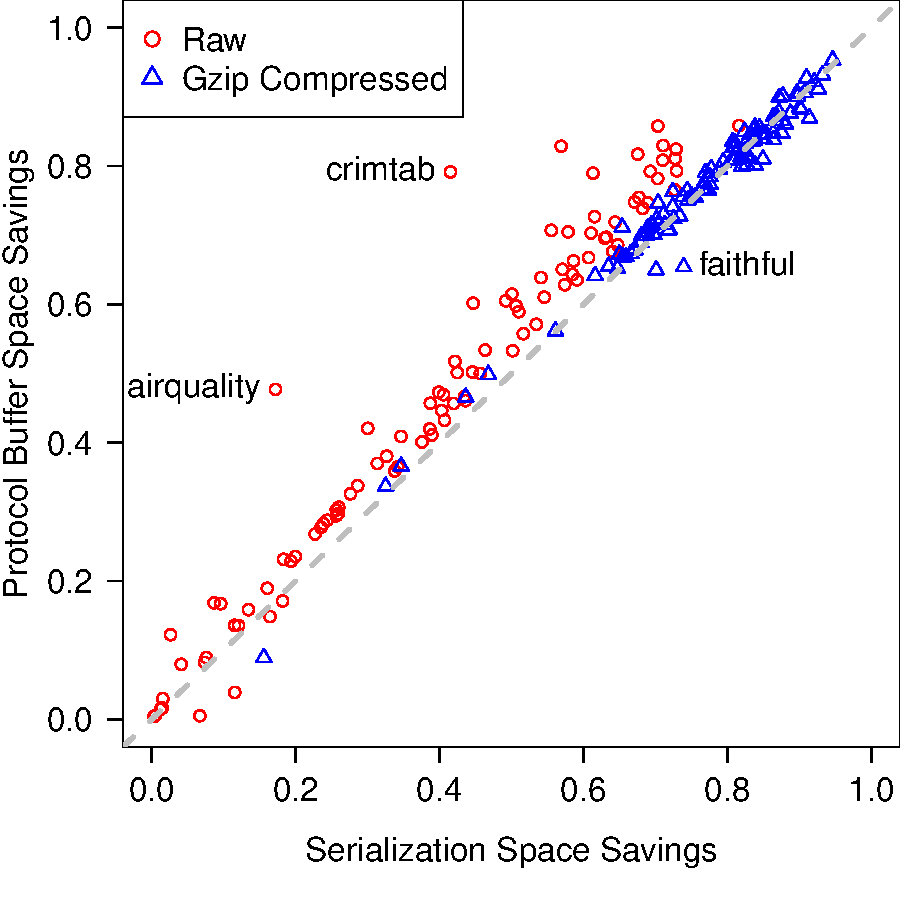
\includegraphics[width=0.45\textwidth]{fig-SER}

\vspace*{0.3cm}

\small
\begin{tabular}{rrrrrrr}
  \hline

  Data set & \code{object.size} & \multicolumn{2}{c}{\proglang{R} serialization} &
  \multicolumn{2}{c}{\pkg{RProtoBuf} serialization} \\
  & & default & gzipped & default & gzipped \\
  \hline
 \code{crimtab} & 7,936 & 4,641 (41.5\%) & 714 (91.0\%) & 1,655 (79.1\%) & 576 (92.7\%)\\
 \code{airquality} & 5,496 & 4,551 (17.2\%) & 1,242 (77.4\%) & 2,874 (47.7\%) & 1,294 (76.4\%)\\
 \code{faithful} & 5,136 & 4,543 (11.5\%) & 1,339 (73.9\%) & 4,936 \phantom{0}(3.9\%) & 1,776 (65.4\%)\\
   \hline
 All & 609,024 & 463,833 (24\%) & 139,814 (77\%) & 436,746 (28\%) & 142,783 (77\%)\\
\hline
\end{tabular}
\caption{(Top) Relative space savings of Protocol Buffers and native \proglang{R} serialization over the raw object sizes of each of the 104 data sets in the \pkg{datasets} package. Points to the left of the dashed $y=x$ line represent datasets that are more efficiently encoded with Protocol Buffers. (Bottom) Absolute space savings of three outlier datasets and the aggregate performance of all datasets.
R version 3.3.1 was used for both the figure and the table. }
\label{fig:compression}
\end{figure}

\section{Application: Distributed data collection with MapReduce}
\label{sec:mapreduce}

Protocol Buffers are used extensively at Google for almost all
RPC protocols, and to store structured information on a variety of
persistent storage systems \citep{dean2009designs}. Since the
initial release in 2010, hundreds of Google's statisticians and
software engineers use the \pkg{RProtoBuf} package on a daily basis
to interact with these systems from within \proglang{R}.
The current section illustrates the power of Protocol Buffers to
collect and manage large structured data in one language 
before analyzing it in \proglang{R}. Our example uses MapReduce
\citep{dean2008mapreduce}, which has emerged in the last
decade as a popular design pattern to facilitate parallel 
processing of big data using distributed computing clusters.

Big data sets in fields such as particle physics and information
processing are often stored in binned (histogram) form in order 
to reduce storage requirements \citep{scott2009multivariate}. 
Because analysis over such large data sets may involve very rare
phenomenon or deal with highly skewed data sets or inflexible
raw data storage systems, unbiased sampling is often not feasible.
In these situations, MapReduce and binning may be combined as a
pre-processing step for a wide range of statistical and scientific
analyses \citep{blocker2013}.

There are two common patterns for generating histograms of large data
sets in a single pass with MapReduce. In the first method, each
mapper task generates a histogram over a subset of the data that it
has been assigned, serializes this histogram and sends it to one or
more reducer tasks which merge the intermediate histograms from the
mappers. In the second method, illustrated in
Figure~\ref{fig:mr-histogram-pattern1}, each mapper rounds a data
point to a bucket width and outputs that bucket as a key and ``1'' as a
value.  Reducers count how many times each key occurs and outputs a
histogram to a data store.

\begin{figure}[t!]
\centering
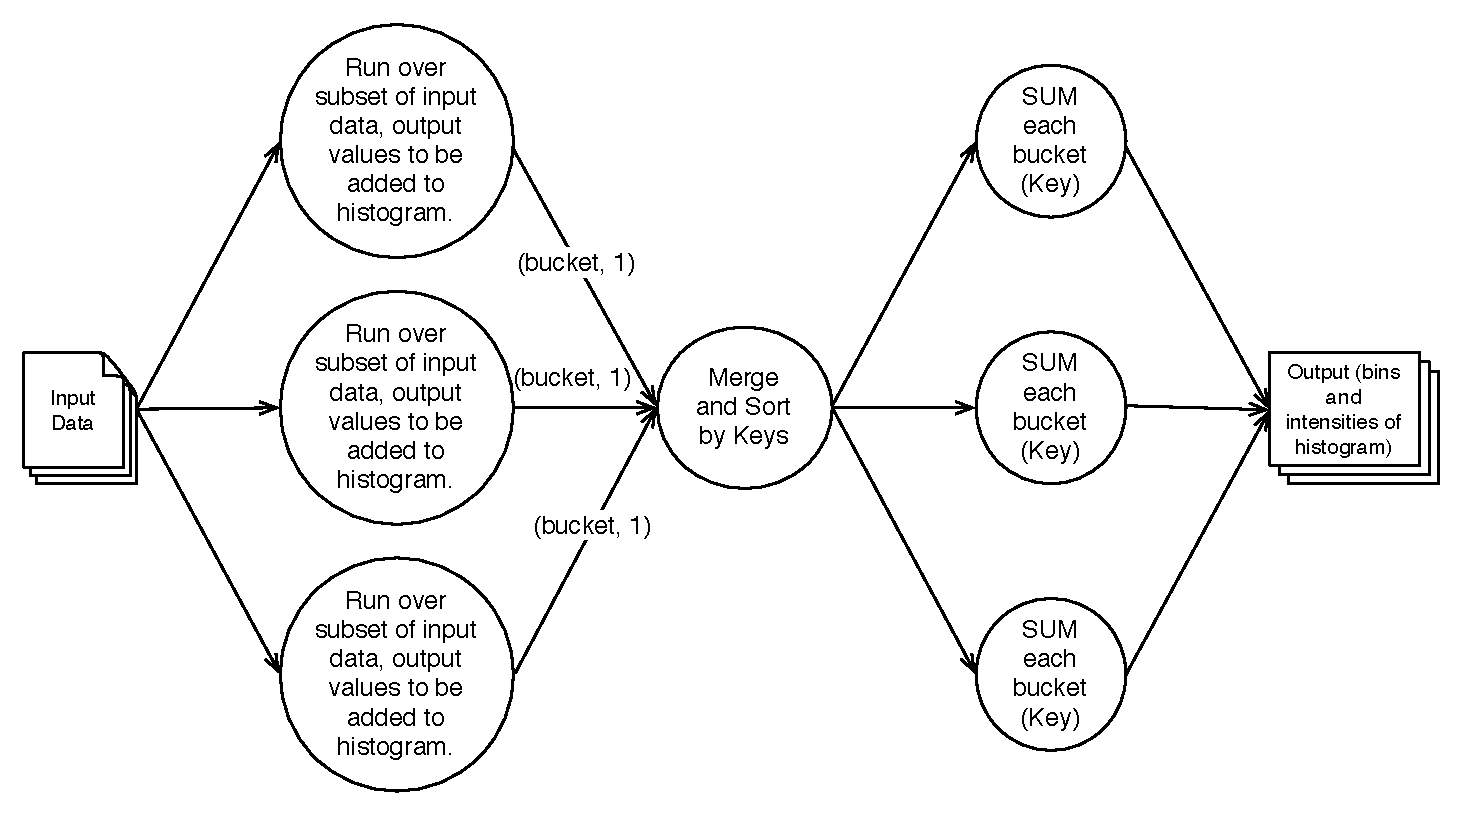
\includegraphics[width=0.9\textwidth]{histogram-mapreduce-diag1.pdf}
\caption{Diagram of MapReduce histogram generation pattern.}
\label{fig:mr-histogram-pattern1}
\end{figure}

In both methods, the mapper tasks must choose identical bucket
boundaries in advance if we are to construct the histogram in a single
pass, even though they are analyzing disjoint parts of the input set
that may cover different ranges.  All distributed tasks involved in
the pre-processing as well as any downstream data analysis tasks must
share a schema of the histogram representation to coordinate
effectively.

The \pkg{HistogramTools} package \citep{histogramtools} enhances
\pkg{RProtoBuf} by providing a concise schema for \proglang{R}
histogram objects:
%
\begin{example}
package HistogramTools;

message HistogramState {
  repeated double breaks = 1;
  repeated int32 counts = 2;
  optional string name = 3;
}
\end{example}
%
This \code{HistogramState} message type is designed to be helpful if
some of the Map or Reduce tasks are written in \proglang{R}, or if
those components are written in other languages and only the resulting
output histograms need to be manipulated in \proglang{R}.

\subsection[A simple single-machine example for Python to R
serialization]{A simple single-machine example for \proglang{Python}
  to \proglang{R} serialization}

To create \code{HistogramState}
messages in \proglang{Python} for later consumption by \proglang{R}, we first compile the 
\code{histogram.proto} descriptor into a python module using the
\code{protoc} compiler:
%
\begin{CodeChunk}
\begin{CodeInput}
protoc histogram.proto --python_out=.
\end{CodeInput}
\end{CodeChunk}
%
This generates a \proglang{Python} module called \code{histogram\_pb2.py}, containing both the 
descriptor information as well as methods to read and manipulate the histogram 
message data.  The following simple \proglang{Python} script uses this generated
module to create a histogram (to which breakpoints and binned data are
added), and writes out the Protocol Buffer
representation to a file:
%
\begin{Code}
from histogram_pb2 import HistogramState;
hist = HistogramState()
hist.counts.extend([2, 6, 2, 4, 6])
hist.breaks.extend(range(6))
hist.name = "Example Histogram Created in Python"
outfile = open("/tmp/hist.pb", "wb")
outfile.write(hist.SerializeToString())
outfile.close()
\end{Code}
%
The Protocol Buffer created from this \proglang{Python} script can
then be read into \proglang{R} and converted to a native \proglang{R}
histogram object for plotting. The code below first attaches the
\pkg{HistogramTools} package which imports \pkg{RProtoBuf}.  Then
reads all of the \code{.proto} descriptor definitions provided by
\pkg{HistogramTools} and adds them to the environment as described in
Section~\ref{sec:rprotobuf-basic}.  Next the serialized Protocol
Buffer is parsed using the \code{HistogramTools.HistogramState}
schema.  Finally the Protocol Buffer representation of the histogram
is converted to a native \proglang{R} histogram object with
\code{as.histogram} and passes the result to \code{plot} (see
Figure~\ref{figure}).
%
\begin{CodeChunk}
\begin{CodeInput}
R> library("HistogramTools")
R> readProtoFiles(package = "HistogramTools")
R> hist <- HistogramTools.HistogramState$read("/tmp/hist.pb")
R> hist
\end{CodeInput}
\begin{CodeOutput}
[1] "message of type 'HistogramTools.HistogramState' with 3 fields set"
\end{CodeOutput}
\begin{CodeInput}
R> plot(as.histogram(hist), main = "")
\end{CodeInput}
\end{CodeChunk}
%
\begin{figure}[t!]
  \centering
  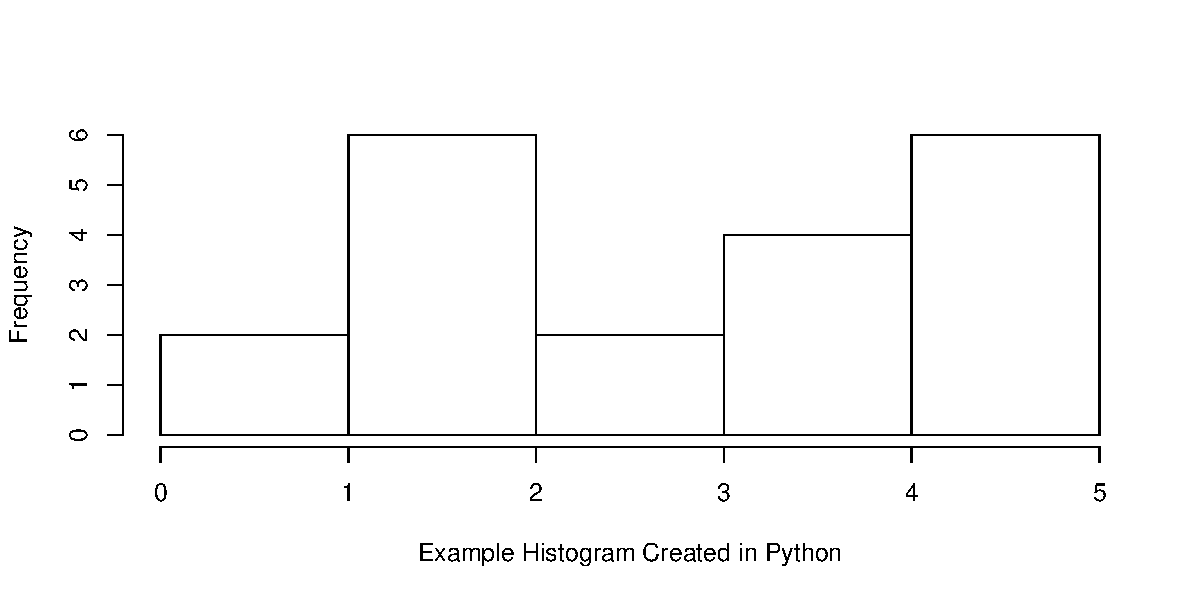
\includegraphics{fig-021}
  \caption{Histogram converted to an \proglang{R} object from \proglang{Python}.}\label{figure}
\end{figure}

This simple example uses a constant histogram generated in
\proglang{Python} to illustrate the serialization concepts without
requiring the reader to be familiar with the interface of any
particular MapReduce implementation.  In practice, using Protocol
Buffers to pass histograms between another programming language and
\proglang{R} would provide a much greater benefit in a distributed
context.  For example, a first-class data type to represent histograms
would prevent individual histograms from being split up and would
allow the use of combiners on Map workers to process large data sets
more efficiently than simply passing around lists of counts and
buckets.

One of the authors has used this design pattern with \proglang{C++}
MapReduces over very large data sets to write out histogram protocol
buffers for several large-scale studies of distributed storage systems
\citep{sciencecloud,janus}.

\section{Application: Data interchange in web services}
\label{sec:opencpu}

The previous section described an application where data from a
program written in another language was saved to persistent storage
and then read into \proglang{R} for further analysis.  This section
describes another common use case where Protocol Buffers are used as
the interchange format for client-server communication.
Network protocols
such as HTTP provide mechanisms for client-server communication, i.e., how to
initiate requests, authenticate, send messages, etc.  However, network
protocols generally do not regulate the \emph{content} of messages: They
allow transfer of any media type, such as web pages, static files or
multimedia content.  When designing systems where various components require
exchange of specific data structures, we need something on top of the network
protocol that prescribes how these structures are to be represented in
messages (buffers) on the network. Protocol Buffers solve this
problem by providing a cross-platform method for serializing arbitrary
structures into well defined messages, which can then be exchanged using any
protocol.

\subsection[Interacting with R through HTTPS and Protocol Buffers]{Interacting with \proglang{R} through HTTPS and Protocol Buffers}

One example of a system that supports Protocol Buffers to interact
with \proglang{R} is \pkg{OpenCPU} \citep{opencpu}. \pkg{OpenCPU} is a framework
for embedded statistical computation and reproducible research based
on \proglang{R} and \LaTeX. It exposes a HTTP(S) API to access and
manipulate \proglang{R} objects and execute remote \proglang{R}
function calls. Clients do not need to understand or generate any
\proglang{R} code: HTTP requests are automatically mapped to function
calls, and arguments/return values can be posted/retrieved using
several data interchange formats, such as Protocol Buffers.  \pkg{OpenCPU}
uses the \code{rexp.proto} descriptor and the \code{serialize\_pb} and
\code{unserialize\_pb} functions described in
Section~\ref{sec:evaluation} to convert between \proglang{R} objects
and Protocol Buffer messages.

\subsection[HTTP GET: Retrieving an R object]{\code{HTTP GET}: Retrieving an \proglang{R} object}

The \code{HTTP GET} method is used to read a resource from
\pkg{OpenCPU}. For example, to access the data set \code{Animals} from the
package \pkg{MASS} \citep{MASS}, a client performs the following HTTP
request:
%
\begin{CodeChunk}
\begin{CodeInput}
GET https://demo.ocpu.io/MASS/data/Animals/pb
\end{CodeInput}
\end{CodeChunk}
%
The postfix \code{/pb} in the URL tells the server to send this
object in the form of a Protocol Buffer message.
% Alternative formats include \code{/json}, \code{/csv}, \code{/rds} and others.
If the request
is successful, \pkg{OpenCPU} returns the serialized object with HTTP status
code 200 and HTTP response header \code{Content-Type: application/x-protobuf}.
The latter is the conventional MIME type that formally notifies the client to
interpret the response as a Protocol Buffer.

Because both HTTP and Protocol Buffers have libraries available for
many languages, clients can be implemented in just a few lines of
code. Below is example code for both \proglang{R} and
\proglang{Python} that retrieves an \proglang{R} data set encoded as a
Protocol Buffer message from \pkg{OpenCPU}.  In \proglang{R}, we use the
HTTP client from the \pkg{httr} package \citep{httr}. In this example
we download a data set which is part of the base \proglang{R}
distribution, so we can verify that the object was transferred without
loss of information.
%
\begin{Schunk}
\begin{Sinput}
R> library("RProtoBuf")
R> library("httr")
R> req <- GET("https://demo.ocpu.io/MASS/data/Animals/pb")
R> output <- unserialize_pb(req$content)
R> identical(output, MASS::Animals)
\end{Sinput}
\end{Schunk}
%
Similarly, to retrieve the same data set in a \proglang{Python} client, we first
compile the \code{rexp.proto} descriptor into a python module
using the \code{protoc} compiler:
%
\begin{CodeChunk}
\begin{CodeInput}
protoc rexp.proto --python_out=.
\end{CodeInput}
\end{CodeChunk}
%
This generates \proglang{Python} module called \code{rexp\_pb2.py}, containing
both the descriptor information as well as methods to read and
manipulate the \proglang{R} object message. We use the
HTTP client from the \code{urllib2} module in our example to retrieve the
encoded Protocol Buffer from the remote server then parse and print it
from \proglang{Python}.
%
\begin{CodeChunk}
\begin{CodeInput}
import urllib2
from rexp_pb2 import REXP
req = urllib2.Request("https://demo.ocpu.io/MASS/data/Animals/pb")
res = urllib2.urlopen(req)
msg = REXP()
msg.ParseFromString(res.read())
print(msg)
\end{CodeInput}
\end{CodeChunk}
%
The \code{msg} object contains all data from the \code{Animals} data
set. From here we can easily extract the desired fields for further
use in \proglang{Python}.

\subsection[HTTP POST: Calling an R function]{\code{HTTP POST}: Calling an \proglang{R} function}

The previous example used a simple \code{HTTP GET} method to retrieve
an \proglang{R} object from a remote service (\pkg{OpenCPU}) encoded as a
Protocol Buffer.
In many cases simple \code{HTTP GET} methods are insufficient, and a
more complete RPC system may need to create compact Protocol Buffers
for each request to send to the remote server in addition to parsing
the response Protocol Buffers.

The \pkg{OpenCPU} framework allows us to do arbitrary \proglang{R} function
calls from within any programming language by encoding the arguments
in the request Protocol Buffer.  The following example \proglang{R}
client code performs the remote function call \code{stats::rnorm(n =
  42, mean = 100)}. The function arguments (in this case \code{n} and
\code{mean}) as well as the return value (a vector with 42 random
numbers) are transferred using Protocol Buffer messages. RPC in
\pkg{OpenCPU} works like the \code{do.call} function in \proglang{R}, hence
all arguments are contained within a list.
%
\begin{Schunk}
\begin{Sinput}
R> library("httr")
R> library("RProtoBuf")
R> args <- list(n = 42, mean = 100)
R> payload <- serialize_pb(args, NULL)
R> req <- POST(url = "https://demo.ocpu.io/stats/R/rnorm/pb", body = payload,
+    add_headers("Content-Type" = "application/x-protobuf"))
R> output <- unserialize_pb(req$content)
R> print(output)
\end{Sinput}
\end{Schunk}
%
The \pkg{OpenCPU} server basically performs the following steps to process the above RPC request:
%
\begin{Schunk}
\begin{Sinput}
R> fnargs <- unserialize_pb(inputmsg)
R> val <- do.call(stats::rnorm, fnargs)
R> outputmsg <- serialize_pb(val)
\end{Sinput}
\end{Schunk}

\section{Summary}  
\label{sec:summary}
Over the past decade, many formats for interoperable
data exchange have become available, each with its unique features,
strengths and weaknesses.  
Text based formats such as CSV and JSON are easy to use, and will likely 
remain popular among statisticians for many years to come. However, in the 
context of increasingly complex analysis stacks and applications involving 
distributed computing as well as mixed language analysis pipelines, choosing a more 
sophisticated data interchange format may reap considerable benefits. 
%Protocol Buffers is itself not a protocol.
%Forward-compatibility is one of the features. No need to re-iterate those 
The Protocol Buffers standard and library offer a unique combination of features, 
performance, and maturity, that seems particularly well suited for data-driven 
applications and numerical computing.

The \pkg{RProtoBuf} package builds on the Protocol Buffers
\proglang{C++} library, and extends the \proglang{R} system with the
ability to create, read, write, parse, and manipulate Protocol Buffer
messages. \pkg{RProtoBuf} has been used extensively inside Google for
the past five years by statisticians, analysts, and software
engineers.  At the time of this writing there are over 300 active
users of \pkg{RProtoBuf} using it to read data from and otherwise
interact with distributed systems written in \proglang{C++},
\proglang{Java}, \proglang{Python}, and other languages. We hope that
making Protocol Buffers available to the \proglang{R} community will
contribute to better software integration and allow for building even
more advanced applications and analysis pipelines with \proglang{R}.

\section*{Acknowledgments}

The first versions of \pkg{RProtoBuf} were written during 2009--2010.
Very significant contributions, both in code and design, were made by
Romain Fran\c{c}ois whose continued influence on design and code is
greatly appreciated. Several features of the package reflect the
design of the \pkg{rJava} package by Simon Urbanek \citep{rjava}.  The
user-defined table mechanism, implemented by Duncan Temple Lang for
the purpose of the \pkg{RObjectTables} package, allows for the dynamic
symbol lookup.  Kenton Varda was generous with his time in reviewing
code and explaining obscure Protocol Buffer semantics.  Karl Millar
and Tim Hesterberg were very helpful in reviewing code and offering
suggestions.  Saptarshi Guha's work on \pkg{RHIPE} and implementation
of a universal message type for \proglang{R} language objects allowed
us to add the \code{serialize_pb} and \code{unserialize_pb} methods
for turning arbitrary \proglang{R} objects into Protocol Buffers
without a specialized pre-defined schema.  Feedback from two anonymous
referees greatly improved both the presentation of this paper and the
package contents.

\bibliography{v71i02}

\begin{appendix}

\section[The rexp.proto schema descriptor]{The \code{rexp.proto} schema descriptor}
\label{rexp.proto}

Below a print of the \code{rexp.proto} schema (originally designed by
\citealt{rhipe}) that is included with the \pkg{RProtoBuf} package and
used by \code{serialize\_pb} and \code{unserialize\_pb}.
%
\begin{CodeChunk}
\begin{CodeInput}
package rexp;
message REXP {
  enum RClass {
    STRING = 0;
    RAW = 1;
    REAL = 2;
    COMPLEX = 3;
    INTEGER = 4;
    LIST = 5;
    LOGICAL = 6;
    NULLTYPE = 7;
    LANGUAGE = 8;
    ENVIRONMENT = 9;
    FUNCTION = 10;
  }
  enum RBOOLEAN {
    F = 0;
    T = 1;
    NA = 2;
  }
  required RClass rclass = 1;
  repeated double realValue = 2 [packed = true];
  repeated sint32 intValue = 3 [packed = true];
  repeated RBOOLEAN booleanValue = 4;
  repeated STRING stringValue = 5;
  optional bytes rawValue = 6;
  repeated CMPLX complexValue = 7;
  repeated REXP rexpValue = 8;
  repeated string attrName = 11;
  repeated REXP attrValue = 12;
  optional bytes languageValue = 13;
  optional bytes environmentValue = 14;
  optional bytes functionValue = 15;
}
message STRING {
  optional string strval = 1;
  optional bool isNA = 2 [default = false];
}
message CMPLX {
  optional double real = 1 [default = 0];
  required double imag = 2;
}
\end{CodeInput}
\end{CodeChunk}

\end{appendix}

\end{document}
